\documentclass[GCT,short]{gct}
	
\usepackage{multirow}
\usepackage{pdfpages}
\usepackage{eurosym}
\usepackage{pdflscape}
\usepackage{subcaption}
%\usepackage{tablenote}
\usepackage{todonotes}
\usepackage{cleveref}

\begin{document}

\title{CHEC Camera MC Params}
\shorttitle{SST2MG-Cam\_MC\_Params} %Replace with 
\acronym{SST2MG-Cam/180424} %Replace 16-06-06 with date (yy-mm-dd)

\version{0.0} %Use 0.X for prerelease, and 1.X for first release etc.
\editor{A. Name}       
\approver{B. Name} %Only use this if applicable, e.g. for an ICD - not
                   %for internal notes etc.            
\comment{Pre-released version}
\distribution{GCT}

\history{
    0.0 & 2018-04-24 & Initial version & GCT & A. Name &  B. Name\\ \hline
}


%%%%% Glossary  %%%%%%%%%%%%%%%%
\newglossaryentry{MAPM}{name={MAPM},description={Multi-Anode Photomultiplier}}

%%%%% DONT CHANGE ! %%%%%%%%%%%%%%%%
\maketitle
\FloatBarrier\if@openright\cleardoublepage\else\clearpage\fi

\maketoc
%%%%%%%%%%%%%%%%%%%%%%%%%%%%%%



\chapter{Camera}

\section{Camera Pixels}
\begin{itemize}
\item Number of pixels per camera.
\item Value adopted: 2048
\item Description of source: By design
\item Status: Agreed
\item Agreed by: T Armstrong, 
\end{itemize}


\section{Camera Config File }

\begin{figure}
\centering
\begin{tabular}{cc}
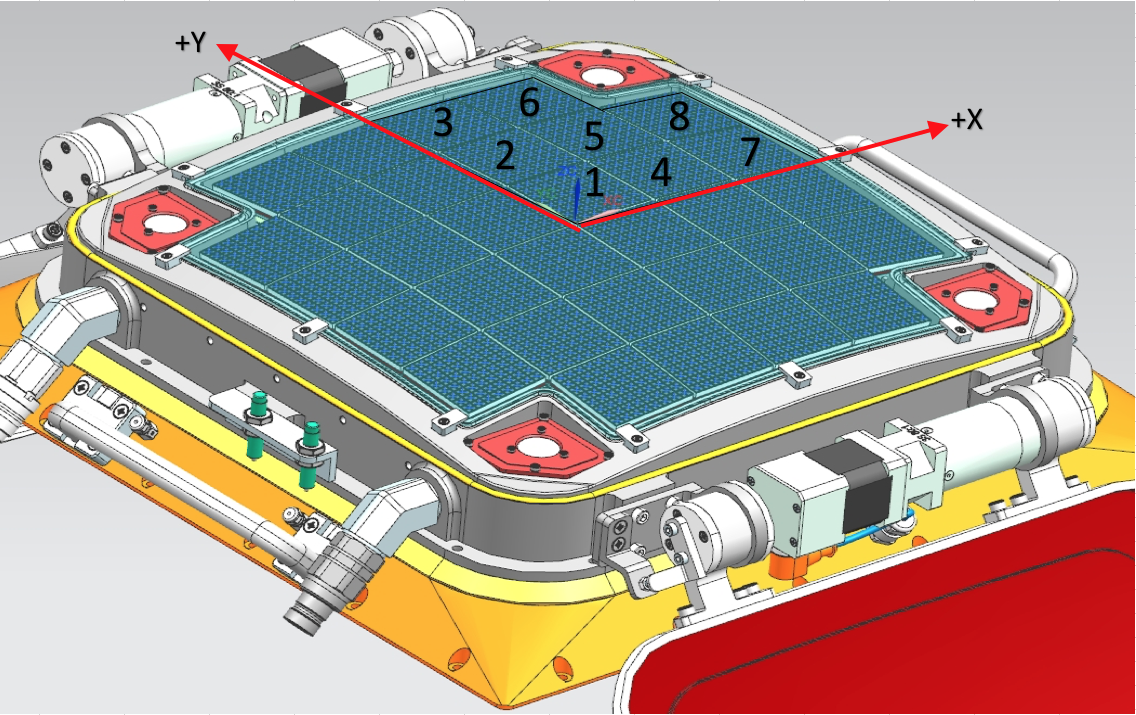
\includegraphics[width=0.55\textwidth]{../02_cameraConfigFile/Picture1.png} & 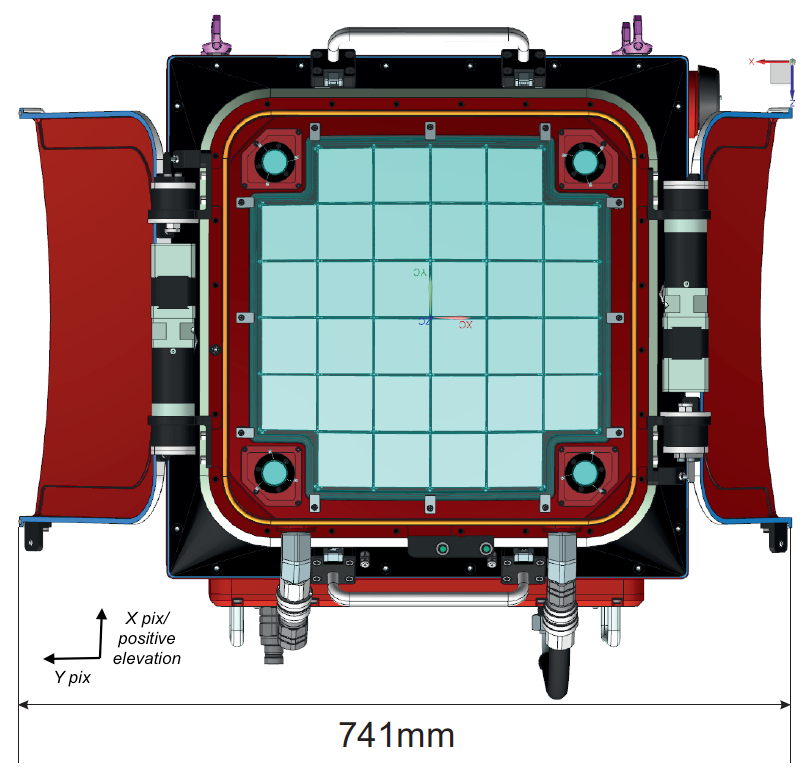
\includegraphics[width=0.40\textwidth]{../02_cameraConfigFile/Picture2.png}  \\
\end{tabular}
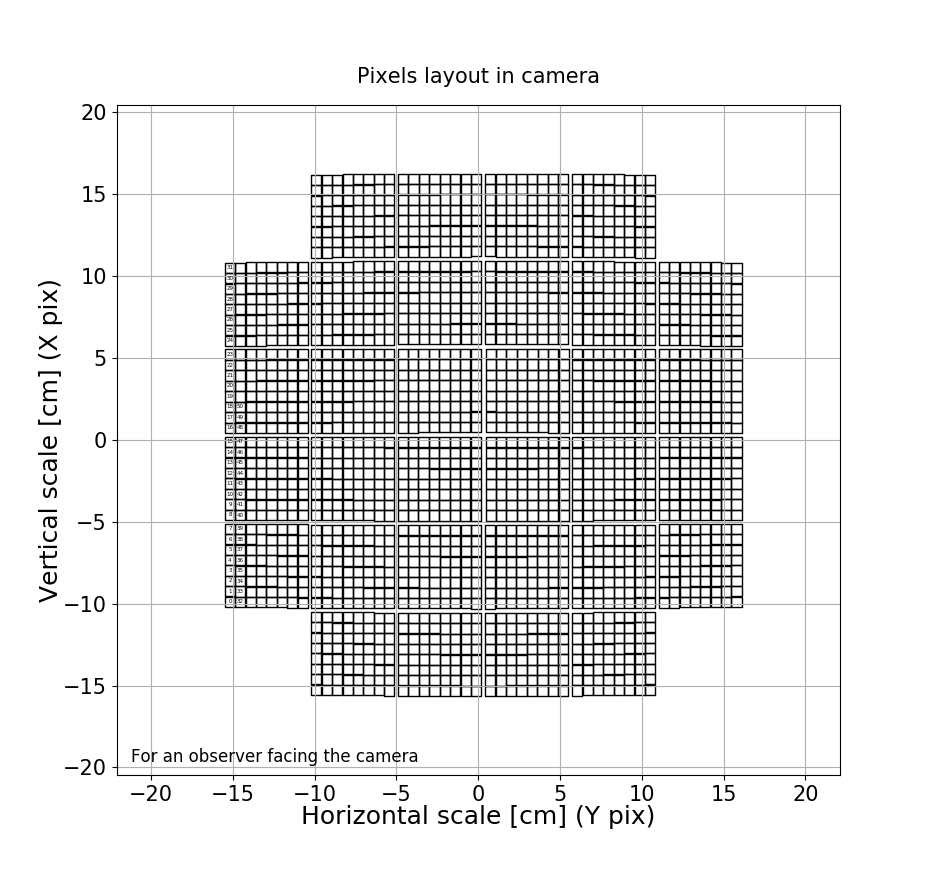
\includegraphics[width=0.69\textwidth]{../02_cameraConfigFile/camera_pixel_layout.png} 
\caption{pixel directions related to the camera focal plane. In the right figure, this represents the focal plane as if you were standing inbetween the camera and the secondary mirror. Therefore, the +ve X direction difined in the configuration file represents +ve elevation from the parked telescope position. The bottotm picture is a plot of the x,y coordinates of the pixels in the updated configuration file.}
\label{fig:focalplane-pixels}
\end{figure}

\begin{figure}
\centering
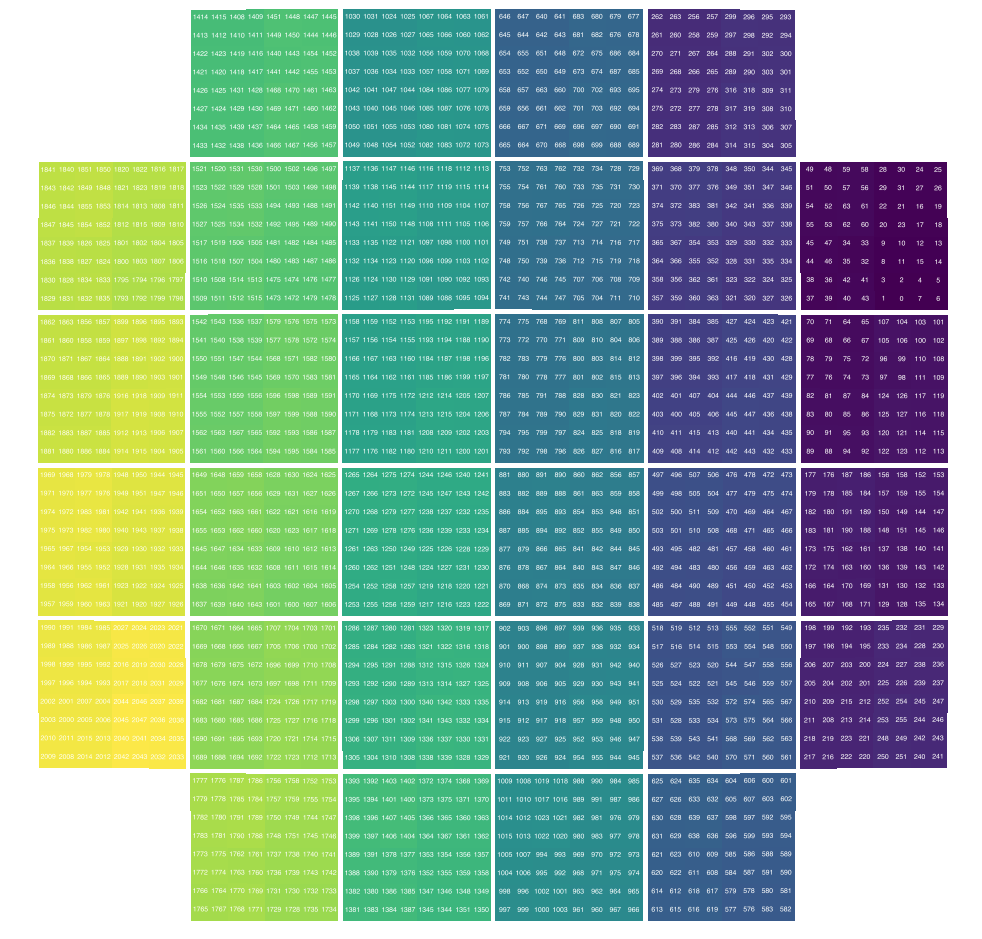
\includegraphics[width=0.75\textwidth]{../02_cameraConfigFile/pixel_mapping.png} \\ 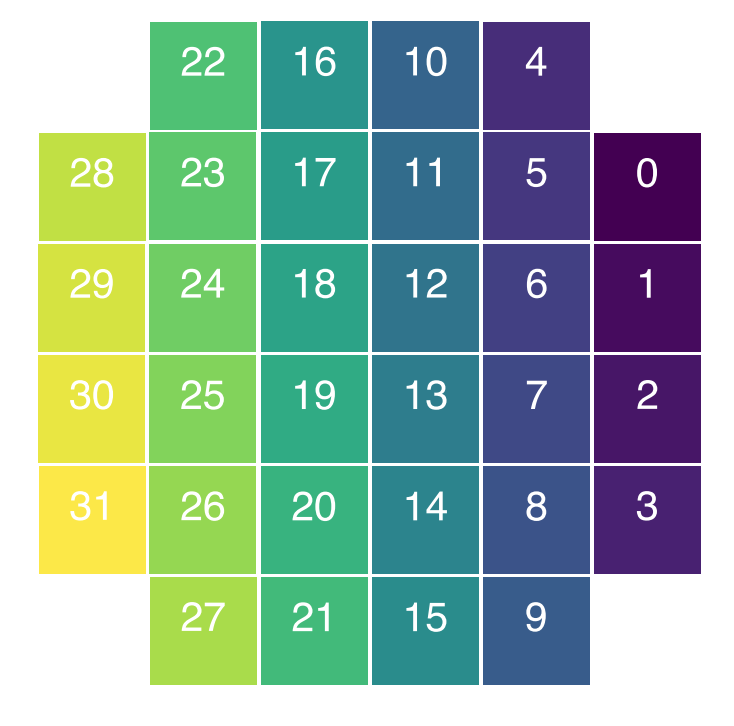
\includegraphics[width=0.5\textwidth]{../02_cameraConfigFile/module_mapping.png}  
\caption{updated pixel (top) and modul (bottom) numbering scheme, such that there is consistency between the camera prototype and the MC model. These values can be found in 02\_cameraConfigFile/ checs\_pixel\_mapping\_v2.txt}
\label{fig:mapping}
\end{figure}



\begin{figure}
\centering
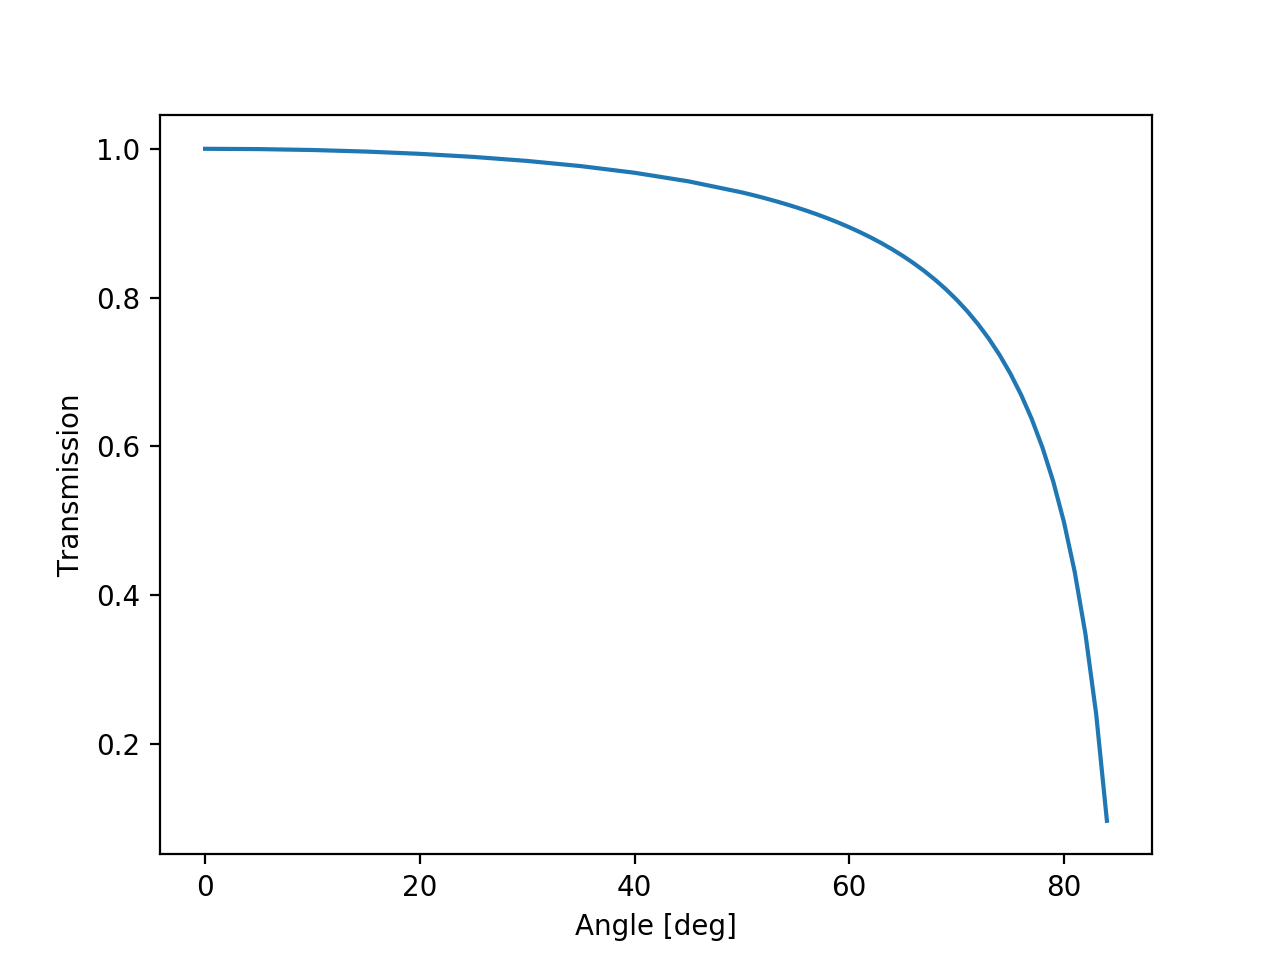
\includegraphics[width=0.65\textwidth]{../02_cameraConfigFile/angleTrans.png}
\caption{Angular transmission of the detectors as used in Prod3.}
\label{fig:trans}
\end{figure}

\begin{itemize}
\item  Configuration file for the description of the camera with pixel types, positions and the circuitry for trigger decisions.
\item Value adopted: checs\_pixel\_mapping\_v2.txt
\item Description of source: 
\begin{itemize}
\item Pixel diameter: \color{red} 0.623 [0.62?] \color{black}- prototype by design
\item Pixel shape:  Square - by design
\item Funnel Shape: same as pixel
\item Funnel Depth: 0 - by design
\item Funnel Diameter: same as pixel
\item Pixel positions: See file 02\_cameraConfigFile/ checs\_pixel\_mapping\_v2.txt, the origional excel file 02\_cameraConfigFile/CHEC-S camera quadrant 512 pixels 19-02-2018-1.xlsx (For reference, on page 1, +X is positive elevation, $\pm$Y is Azimuth, Z is optical axis) and Figure \ref{fig:focalplane-pixels}, output from CAD design model (extracted by Duncan Ross - University of Leicester). The rotation of the camera is important as there is a slight asymmetry in the pixel layout. The mapping has been corrected by Jason Watson to match that used in the camera which can be seen in Fig \ref{fig:mapping}.
\item transmission$(\lambda)$:  None - Moved to seperate parameter: Camera Filter(41)
\item transmission$(\theta)$: transmission\_pmma\_vs\_theta\_20150422.dat [\color{red} NEEDS UPDATING?\color{black} ] See Figure \ref{fig:trans}
\end{itemize}
\item Status: \color{orange}awaiting agreement\color{black}
\item Agreed by: 
\end{itemize}



\section{NSB}
\begin{itemize}
\item Number of photo-electrons per nanosecond per pixel due to nightsky background. Note that the number here takes into account all photo-electrons, including those not properly amplified or lost at the first dynode. A range of pixels can be given with nightsky background = (0-1236): 0.2, (1237-1854): 0.15. Alternatively, all pixels can be set with nightsky background = all: 0.2.
\item Value adopted: 
\item Description of source: 
\item Status: To be derived at end
\item Agreed by: 
\end{itemize}



\section{SPE}

\begin{figure}[h!]
\centering
\begin{tabular}{cc}
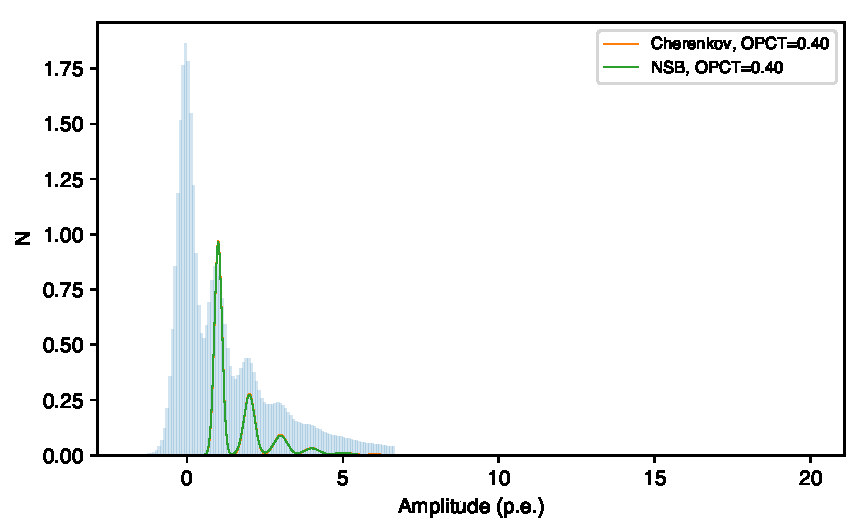
\includegraphics[width=0.5\textwidth]{../04_SPE/checs_spe_spectrum_v2.pdf} & 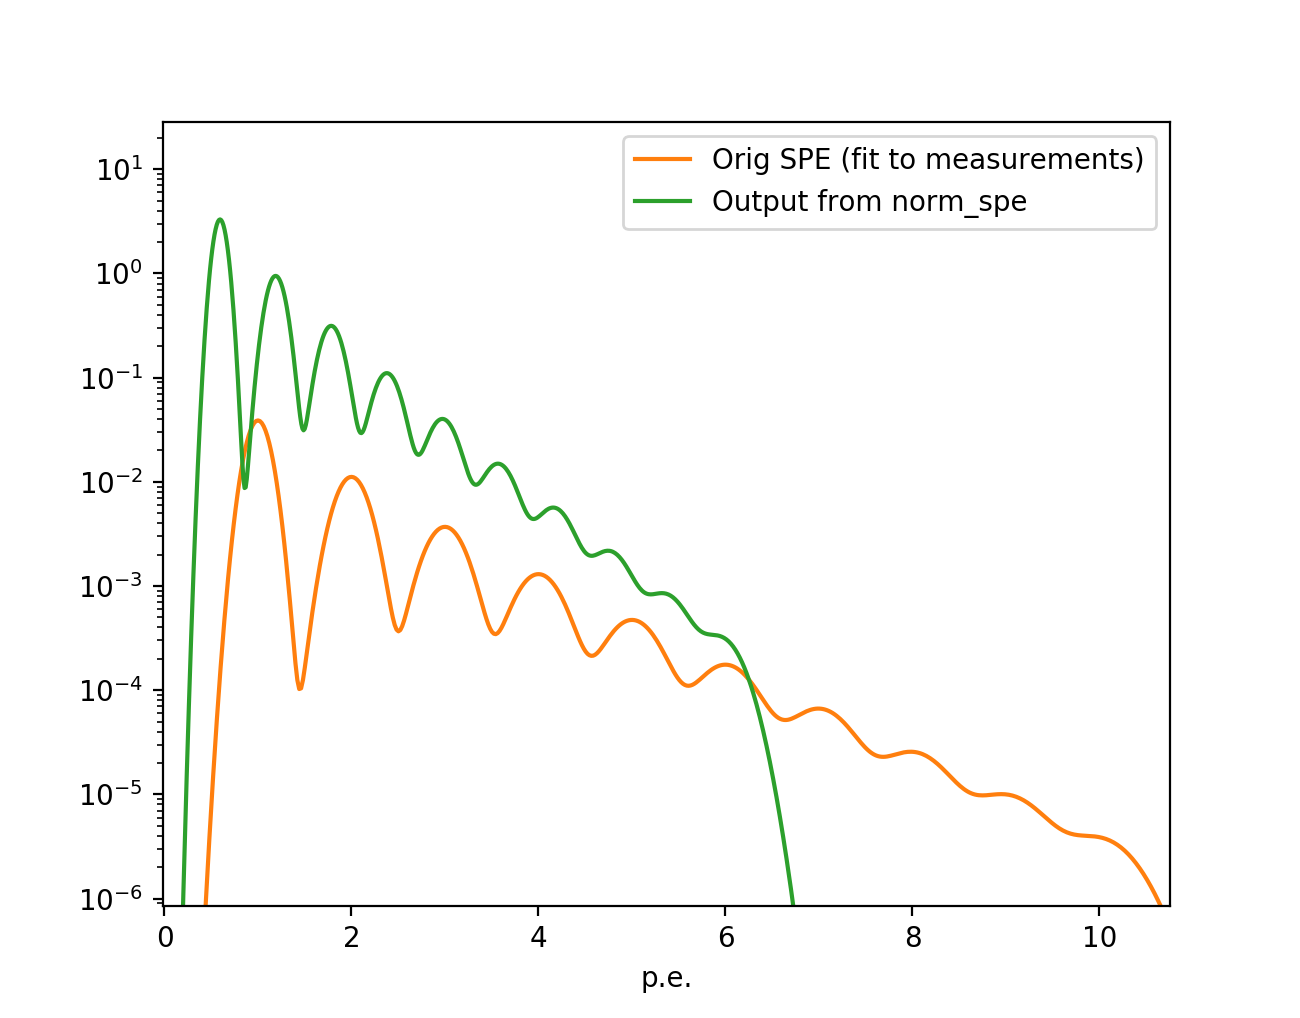
\includegraphics[width=0.45\textwidth]{../04_SPE/SPEnorm_v2.png}  \\
\end{tabular}
\caption{Left: SPE curve for CHEC-S, where the histogram shows the lab measurements and the green and orange line the parameterised fit (exluding the pedistal). Right, the normalised spe curve (orange) required by sim\_telarray (The c.o.g. of the spe distribution must be at 1.0 after normalising)}
\label{fig:spe}
\end{figure}

\begin{itemize}
\item File name for single p.e. response distribution.
\item Value adopted: 04\_SPE/checs\_spe\_spectrum\_v2\_normalised.txt
\item Description of source: See Figure \ref{fig:spe}. \color{red} X Needs data description \color{black}. The fit to the data is then normalised such that the c.o.g. of the distribrution is at 1.0, as is required by sim\_telarray (this was performed using the sscript norm\_spe which is available with the corsika\_simtel package)
\item Status: \color{orange}awaiting agreement\color{black}
\item Agreed by: 
\end{itemize}

\section{Gain Variation }

\begin{figure}[h!]
\centering
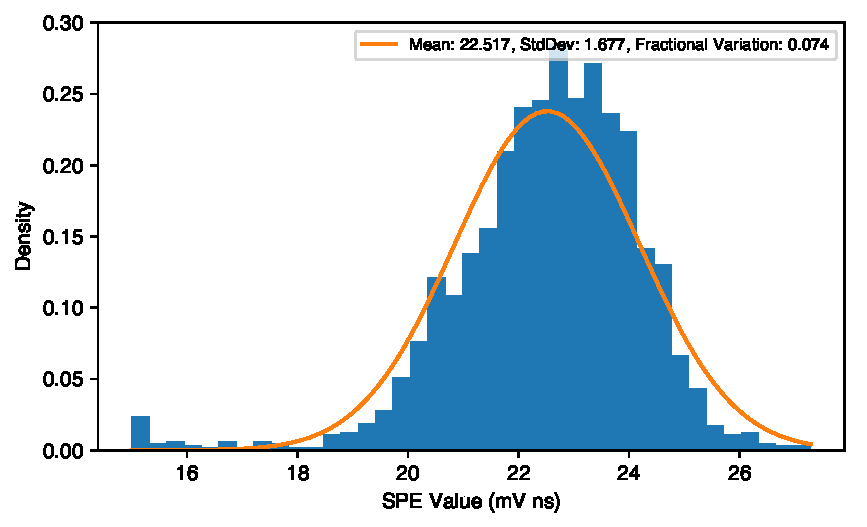
\includegraphics[width=0.65\textwidth]{../05_gainVariation/checs_gain_variation_v2.pdf}
\caption{Gain variation between pixels, i.e. how the p.e. value changes between pixels.}
\label{fig:gainvar}
\end{figure}

\begin{itemize}
\item Fractional gain variation between different photodetectors after adjusting the voltage to have approximately the same gain in all channels. The parameter sets the Gaussian r.m.s. spread of random fluctuations.
\item Value adopted: 10\%
\item Value adopted V2: 7.4\%
\item Description of source:  See Figure \ref{fig:gainvar}. \color{red} X Needs data description \color{black}
\item Status: \color{orange}awaiting measurement\color{black}
\item Agreed by: 
\end{itemize}


\section{PM Voltage Variation}
\begin{itemize}
\item Fractional high voltage variation, used to adjust the transit times (/ 1=p(V )). The parameter sets the Gaussian r.m.s. spread of random voltage fluctuations..
\item Value adopted: 0 
\item Description of source: Does not apply to SiPMs
\item Status: \color{orange}awaiting agreement\color{black}
\item Agreed by: T Armstrong,
\end{itemize}

\section{PM Transit Time}
\begin{itemize}
\item Total transit time of the photodetector at the average voltage.
\item Value adopted: 4ns
\item Description of source: Since PM Voltage Variation is set to zero, this is irrelevant
\item Status: \color{orange}awaiting agreement\color{black}
\item Agreed by: T Armstrong
\end{itemize}

\section{PM Transit Time Jitter}
\begin{itemize}
\item Jitter (Gaussian r.m.s. spread of random fluctuations) of individual photo-electrons in nanoseconds.
\item Value adopted: 
\item Description of source: 
\item Status: \color{red}awaiting measurement\color{black}
\item Agreed by: 
\end{itemize}

\section{Photon Delay}
\begin{itemize}
\item An additional delay added to the arrival times of all photons at the photosensors.
\item Value adopted: 5ns
\item Description of source: Technical MC parameter to place the pulse shape in the simulation time, no need to measure
\item Status: \color{orange}awaiting agreement\color{black}
\item Agreed by: T Armstrong
\end{itemize}

\section{QE}

\begin{figure}[h!]
\centering
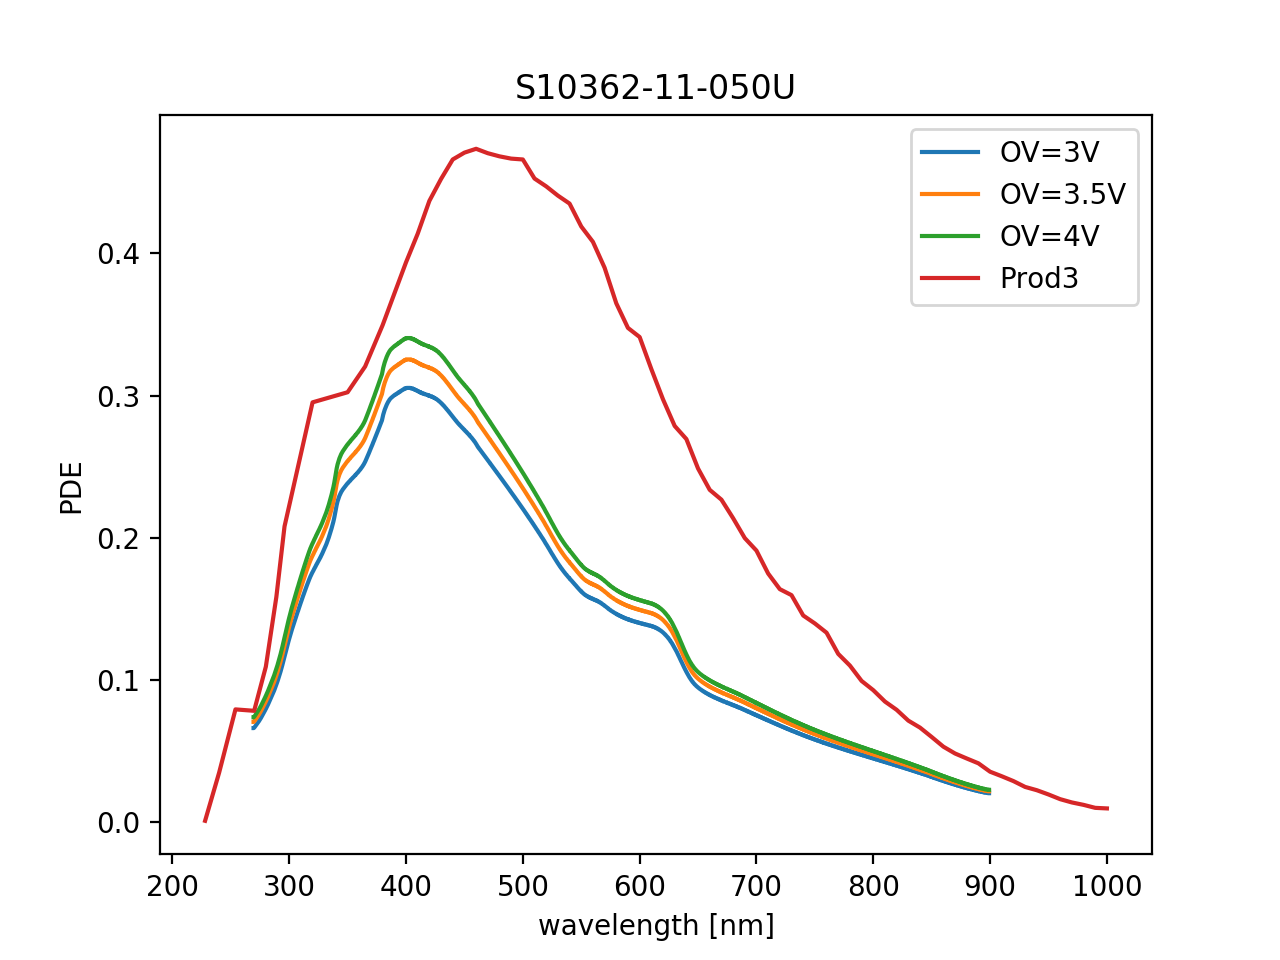
\includegraphics[width=0.65\textwidth]{../10_quantumEfficiency/pde_S10362-11-050U-scaled.png}
\caption{Quantum efficiency for device S10362-11-050U, a similar device to that used in CHEC-S, shown scaled by different overvoltages.}
\label{fig:pde}
\end{figure}

\begin{itemize}
\item File name for the quantum efficiency curve.
\item Value adopted: 10\_quantumEfficiency/S10362-11-050U-3V.txt (prototype!)
\item Description of source: Data provided by Hiro Tajima, data from data sheet(?) for similar device (S10362-11-050U) to that used in CHEC-S (S12642-1616PA) scaled for different OV, see Figure \ref{fig:pde}. Updated measurements being performed in US by Nepomuk and Co.
\item Status: \color{orange}awaiting agreement\color{black}
\item Agreed by: 
\end{itemize}


\section{QE Variations}

\begin{figure}[h!]
\centering
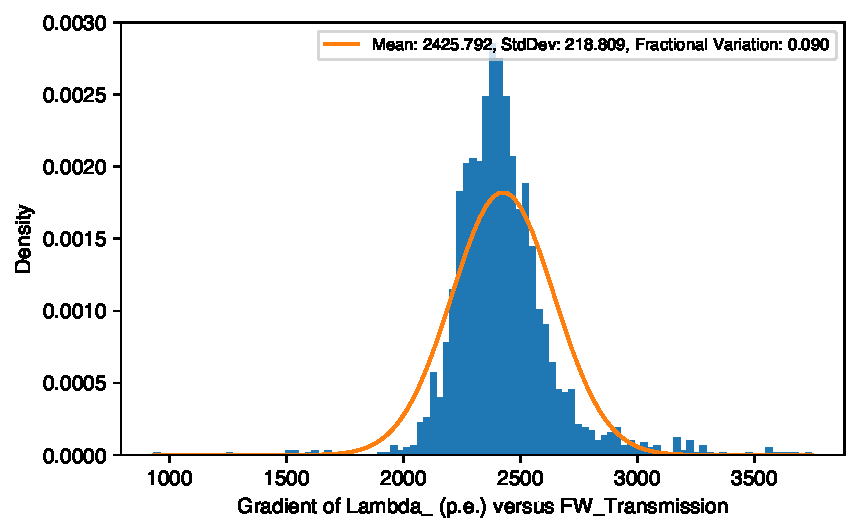
\includegraphics[width=0.65\textwidth]{../11_qeVariation/checs_qe_variation_v2.pdf}
\caption{Quantum efficiency variation}
\label{fig:qevar}
\end{figure}

\begin{itemize}
\item Photoelectron collection efficiency variation (Gaussian r.m.s. spread of random fluctuations) between photodetectors.
\item Value adopted: 10\%
\item Value adopted V2: 9\%
\item Description of source: See Figure \ref{fig:qevar}. Calculated using the gradient of the lambda (illumination at each filter wheel) gradient, gives relative QE efficiency between pixels. \color{red} X Needs data description \color{black}
\item Status:\color{orange} awaiting measurement\color{black}
\item Agreed by: 
\end{itemize}

\section{Disc Bins }
\begin{itemize}
\item Number of time bins used for the discriminator/comparator simulation. The trigger simulation might cover a larger time window than the FADC signals.
\item Value adopted: 120 Time bins
\item Description of source: 
\item Status: \color{red} Needs description \color{black}
\item Agreed by: 
\end{itemize}

\section{Disc Start}
\begin{itemize}
\item Number of time bins by which the discriminator/comparator simulation is ahead of the FADC readout.That is mainly relevant if different time windows are simulated for comparator inputs and digitised ADC values.
\item Value adopted: 3
\item Description of source: 
\item Status: \color{red} Needs description \color{black}
\item Agreed by: 
\end{itemize}


\section{Default Trigger}
\begin{itemize}
\item The default meaning of a “Trigger” line in the camera definition file. If set to “Majority”, a “Trigger” line would indicate a “MajorityTrigger”, for “AnalogSum” it would indicate an “AnalogSumTrigger”,and for “DigitalSum” it would indicate a “DigitalSumTrigger”.
\item Value adopted: Majority
\item Description of source: By design, at the end of the camera configuration file (2) there is the definitions of the trigger patches, this includes the ``super pixel" (majority sum of a patch of 4 pixels). This has remained unchanged since $\sim$2013. See diagrnostic plot, Figure \ref{fig:triggerpattern}, to see that the pixel numbering and the definistion of the majority trigger of super pixels are still consitent.
\item Status: \color{orange} Awaiting agreement\color{black}
\item Agreed by: T Armstrong,
\end{itemize}


\begin{figure}
\centering
\begin{tabular}{cc}
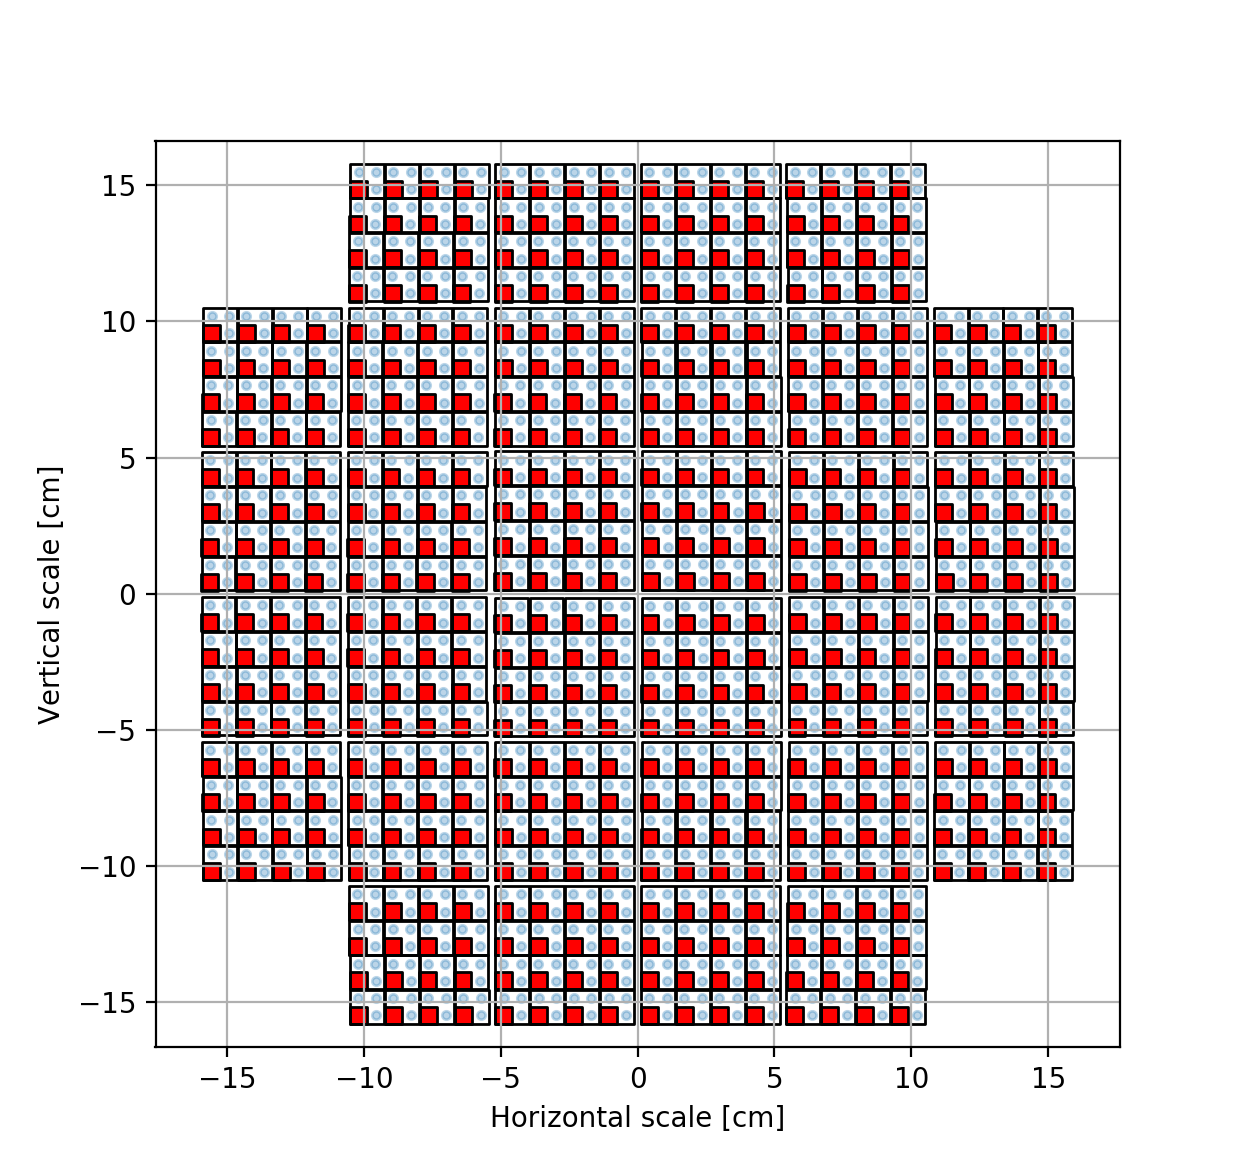
\includegraphics[width=0.51\textwidth]{../14_defaultTrigger/super_pixels.png} & 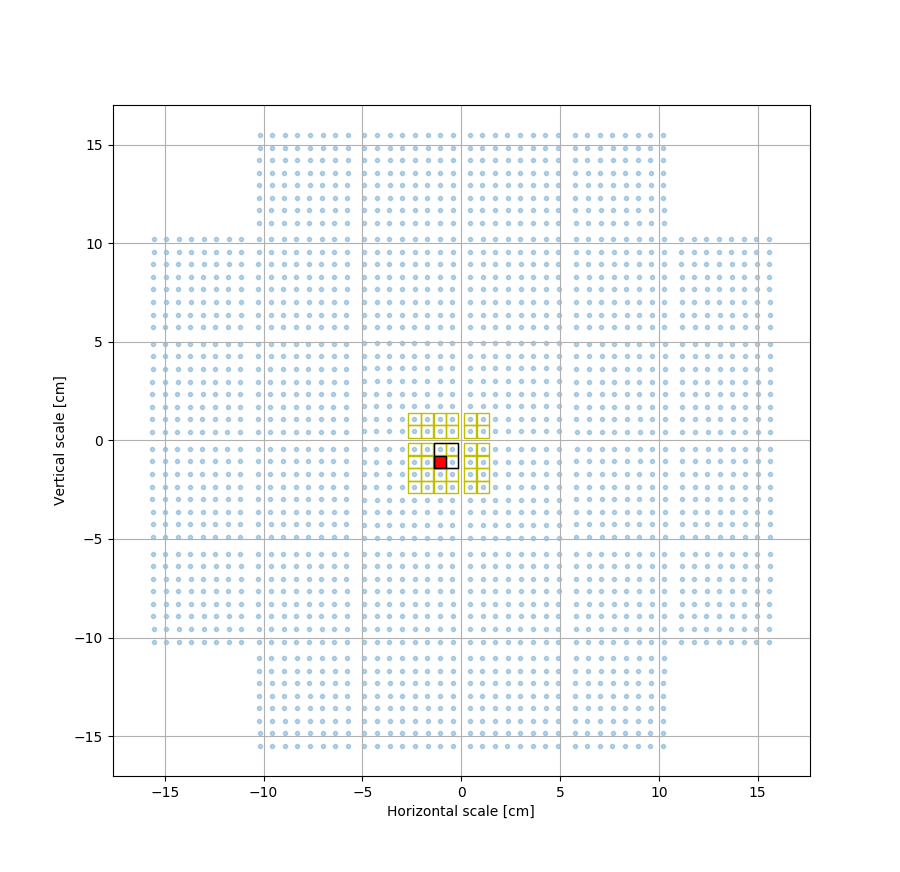
\includegraphics[width=0.5\textwidth]{../14_defaultTrigger/super_pixel_neighbours.png} \\
\end{tabular}
\caption{Left: Definition of the Majority sum of 4 neighbouring pixels within the camera configuration (2). Where the super pixels are defined as $n_1 [n_2,n_3,n_4]$, the figure displays the first pixel (red) and then the combination of all (black squares). Right: Surounding super-pixel pixels within which to search for a coincidence (i.e. a 3x3 grid of super pixels). }
\label{fig:triggerpattern}
\end{figure}


\section{Pulse Shape}
\begin{itemize}
\item File name for pulse shape at the discriminator/comparator of an individual pixel. (DISC)
\item Value adopted: 15\_pulseShape/disc\_shape\_CHEC-S\_27042018.dat and 15\_pulseShape/pulse\_CHEC-S\_FADC\_27042018.dat
\item Description of source:  pulse shape measured in Leicester using a LeCroy scope on the output of the prototype shaper boards using the CHEC-S SiPMs. The prototype shaper is 2 channel test board with unrepresentative layout but  using the final component values. This was before the new TARGET boards were available. The origional data is provided in 15\_pulseShape/pulse\_data.txt but has had the leading baseline removed, has been normalised to a maximum of 1 and has been written out to the required format for the Discriminator and FADC pulse shapes. See Figure \ref{fig:pulse-shape}, including the prod3 pulse shape for reference. Data provided by Jon Lapington in Leicester.
\item Status: \color{orange}Awaiting agreement\color{black}
\item Agreed by: T Armstrong, 
\end{itemize}

\begin{figure}
\centering
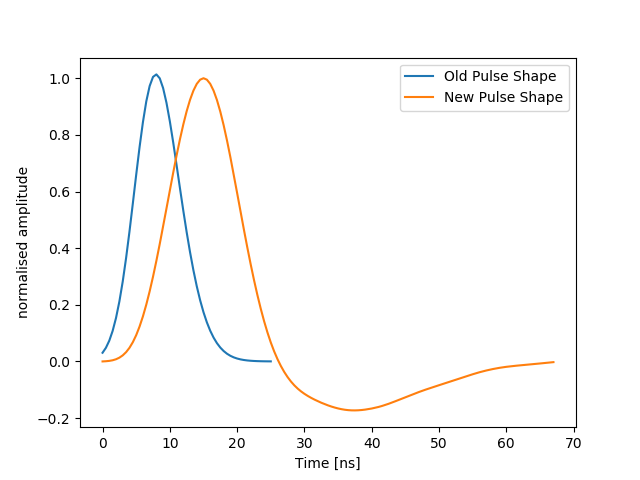
\includegraphics[width=0.55\textwidth]{../15_pulseShape/pulse_shape_comparison.png} 
\caption{Pulse shape for CHEC-S, measured in Leicester.}
\label{fig:pulse-shape}
\end{figure}

\section{Discriminator Amplitude}
\begin{itemize}
\item Signal amplitude after amplifier per mean p.e. at the input of the discriminators/comparators. The unit is arbitrary (typically mV) but the same definition has to be used for the discriminator threshold. For the default value of 1.0, the unit is the average (not the most probable) amplitude of a single photo-electron, implying the same being used for thresholds and switching behaviour.
\item Amendment, due to the normalisation of the SPE curve, this might need reconsidering. 
\item Value adopted: 1 (changed from 20)
\item Description of source: Desire to have in units of p.e., for CHEC, only relevant to disc\_threshold.
\item Status: \color{orange}Awaiting check\color{black}
\item Agreed by: 
\end{itemize}


\section{Trigger Pixels }
\begin{itemize}
\item Number of pixels required for single telescope trigger. With flexible camera definitions, this is the default number for the multiplicity required per trigger group. If the camera definition file contains a non-zero number in the definition of any trigger group, that number overrides the default
\item Value adopted: 2
\item Description of source: Current design implementation, this means a minimum of 2 ``super-pixels" are required to be in coincidence for a trigger. These must be neighbouring pixels (see Figure \ref{fig:triggerpattern}, the neighbouring pixels would be required to be in the highlighted pixels in the right figure).
\item Status: \color{orange}Awaiting agreement\color{black}
\item Agreed by: T Armstrong, 
\end{itemize}


\section{Teltrig Min Time}
\begin{itemize}
\item Minimum time of sector trigger over threshold. Used before telescope trigger.
\item Value adopted: 
\item Description of source: 
\item Status: \color{red}awaiting measurement\color{black}
\item Agreed by: 
\end{itemize}


\section{Teltrig Min Sigsum}
\begin{itemize}
\item Minimum signal sum at sector trigger over threshold. Note that both the minimum time over threshold and the minimum signal sum have to be satisfied before a trigger is obtained. Normally, either of these values being non-zero should be sufficient.
\item Value adopted: 0
\item Description of source: By design, do not consider the integrated signal of the trigger line.
\item Status: \color{orange}Awaiting agreement\color{black}
\item Agreed by: T Armstrong, 
\end{itemize}


\section{Discriminator Sigsum Over Thresh }
\begin{itemize}
\item Integrated signal required over threshold. See also discriminator time over threshold above for combined effects. If discriminator time over threshold is not milliVolts, it scales accordingly.
\item Value adopted: 0
\item Description of source: By design, do not consider the integrated signal of the trigger line.
\item Status: \color{orange}Awaiting agreement\color{black}
\item Agreed by: T Armstrong, 
\end{itemize}


\section{Discriminator Var Sigsum over Thresh}
\begin{itemize}
\item Gaussian r.m.s. spread of discriminator sigsum over threshold (Pixel-to-pixel variation).
\item Value adopted: 0 
\item Description of source: By design, do not consider the integrated signal of the trigger line.
\item Status: \color{orange}Awaiting agreement\color{black}
\item Agreed by: T Armstrong, 
\end{itemize}


\section{Discriminator Gate Length}
\begin{itemize}
\item Effective discriminator gate length. To achieve a comparator-type response this gate length must match the time over threshold below.
\item Value adopted: -8 
\item Description of source: Changed to include negative sign, this ensures that the signal drops after 8ns even if the actual signal continues.
\item Status: \color{orange}Awaiting agreement\color{black}
\item Agreed by: T Armstrong
\end{itemize}


\section{Discriminator Var Gate Length}
\begin{itemize}
\item Variation of gate length (Gaussian r.m.s.). In comparator-type response, this variable is not used but only discriminator var time over threshold.
\item Value adopted: 
\item Description of source: 
\item Status: \color{red}awaiting measurements\color{black}
\item Agreed by: 
\end{itemize}


\section{Discriminator Rise Time}
\begin{itemize}
\item Rise time of the discriminator/comparator output. After the discriminator/comparator logical output is set true, the output signal linearly rises from 0 to 100\% within the given time period.
\item Value adopted: 0
\item Description of source: digital pulse
\item Status: \color{orange}Awaiting agreement\color{black}
\item Agreed by: T Armstrong
\end{itemize}


\section{Discriminator Var Threshold}
\begin{itemize}
\item Channel-to-channel variations (random Gaussian r.m.s.) of discriminator/comparator threshold.
\item Value adopted: 
\item Description of source: 
\item Status: \color{red}awaiting measurement\color{black}
\item Agreed by: 
\end{itemize}


\section{Discriminator Hysteresis}
\begin{itemize}
\item The switching off of a comparator is normally with some hysteresis to avoid oscillating behaviour. As a consequence, the signal has to be below the threshold minus the hysteresis before it switches off.
\item Value adopted: 
\item Description of source: 
\item Status: \color{red}awaiting measurement?\color{black}
\item Agreed by: 
\end{itemize}


\section{Discriminator Fall Time}
\begin{itemize}
\item Fall time of discriminator/comparator output after the logical output is reset to false.
\item Value adopted: 0
\item Description of source: digital pulse
\item Status: \color{orange}Awaiting agreement\color{black}
\item Agreed by: T Armstrong, 
\end{itemize}


\section{Discriminator Time Over Thresh}
\begin{itemize}
\item Time over threshold required before logic response switches to true. To achieve a comparator-type response this time must match the gate length above. Note that in addition a minimum signal integral discriminator sigsum over threshold may be set up. If so, both time over threshold and signal integral conditions have to be met before a ‘true’ output signal starts. Normally, either of them being non-zero should be sufficient.
\item Value adopted: 
\item Description of source: 
\item Status: \color{red}awaiting measurement\color{black}
\item Agreed by: 
\end{itemize}


\section{Disc Var Time Over Threshold}
\begin{itemize}
\item Pixel-to-pixel variation of the time over threshold required before logic response switches to true.
\item Value adopted: 
\item Description of source: 
\item Status: \color{red}awaiting measurement\color{black}
\item Agreed by: 
\end{itemize}


\section{Discriminator Output Amplitude}
\begin{itemize}
\item The nominal output amplitude of a pixel discriminator or comparator as seen at the sector (trigger group) coincidence unit.
\item Value adopted: 1
\item Description of source: arbitrary value, set to 1 in the discriminator is binary with a variance of zero
\item Status: \color{orange}Awaiting agreement\color{black}
\item Agreed by: T Armstrong, 
\end{itemize}

\section{Discriminator Output Var Percent}
\begin{itemize}
\item Channel-to-channel variation (Gaussian r.m.s.) of the output amplitude of a pixel discriminator or comparator.
\item Value adopted: 0
\item Description of source: discriminator is binary with a variance of zero.
\item Status: \color{orange}Awaiting agreement\color{black}
\item Agreed by: T Armstrong, 
\end{itemize}

\section{FADC MHz}
\begin{itemize}
\item FADC sampling rate. A value of 250 (MHz or million samples per second) corresponds to an FADC time interval of 4 ns.
\item Value adopted: 1000 MHz
\item Description of source: By design
\item Status: \color{orange}Awaiting agreement \color{black}
\item Agreed by: T Armstrong, 
\end{itemize}

\section{FADC Bins }
\begin{itemize}
\item Number of FADC bins to be filled. In the first place this means the number of bins simulated. The median of all Cherenkov light photo-electrons will be near 40\% of the interval length, unless shifted with photon delay. If the photon delay is left at 0, this will also be used as the number of bins read out.
\item Value adopted: 128 or ...
\item Description of source: To be determined, 128 is fine if useing FADC sum bins of 96, if using 128 then FADC Bins needs to be increased.
\item Status: \color{orange}Awaiting confirmation \color{black}
\item Agreed by: 
\end{itemize}

\section{FADC Sum Bins }
\begin{itemize}
\item Number of bins summed up in ADC sum data or read out in sampled data. This number corresponds to the experimental length of the readout window. The start of the readout window starts fadc sum offset bins before the calculated time of the trigger, as long as the readout window fits fully in the simulated window. With peak sensing readout, the same interval is used for searching the peak signal.
\item Value adopted: 96 or 128?
\item Description of source: A tunable parameter
\item Status: \color{orange}Awaiting confirmation \color{black}
\item Agreed by: 
\end{itemize}

\section{FADC Sum Offset }
\begin{itemize}
\item Number of bins before telescope trigger where summing/reading of sampled data starts (see also description of fadc sum bins). With peak sensing readout, the same offset is used for setting the interval for the searching of the peak signal. For negative values, the summing/reading starts after the trigger.
\item Value adopted: 24
\item Description of source: 
\item Status: \color{red}awaiting desciption\color{black}
\item Agreed by: 
\end{itemize}

\section{36. FADC Pedestal }
\begin{itemize}
\item Nominal (F)ADC pedestal value per time slice.
\item Value adopted: 
\item Description of source: Needs measuring, although can set at a level such that the saturation of the undershoot is replicated in sim\_telarray at large illuminations? 
\item Status: \color{red}Awaiting measurement?\color{black}
\item Agreed by: 
\end{itemize}

\section{FADC Amplitude }

\begin{figure}
\centering
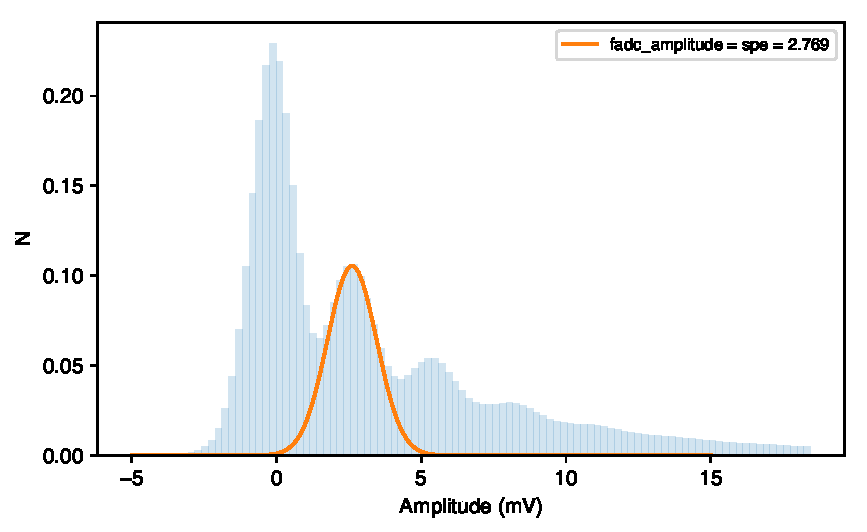
\includegraphics[width=0.55\textwidth]{../37_fadcAmplitude/checs_fadc_amplitude_v2.pdf} 
\caption{FADC Amplitude, measured from the height of the first p.e. peak}
\label{fig:fadcamp}
\end{figure}

\begin{itemize}
\item Peak amplitude at ADC/FADC (for high gain channel, if different gains are used). fadc amplitude are ADC counts maximum amplitude above pedestal (per time slice) for a photo-electron with average (not most probable) signal. This is after photodetector, preamplifier, cable, and shaper at the input of the ADC or FADC.
\item Amendment, due to SPE normalisation this might need checking
\item Value adopted: 2.5
\item Value adopted V2: 2.77
\item Description of source: See Figure \ref{fig:fadcamp}. Value measured from the first peak of the spe. \color{red} X Needs data description \color{black}
\item Status: \color{red}Awaiting check\color{black}
\item Agreed by: 
\end{itemize}

\section{FADC Noise }

\begin{figure}
\centering
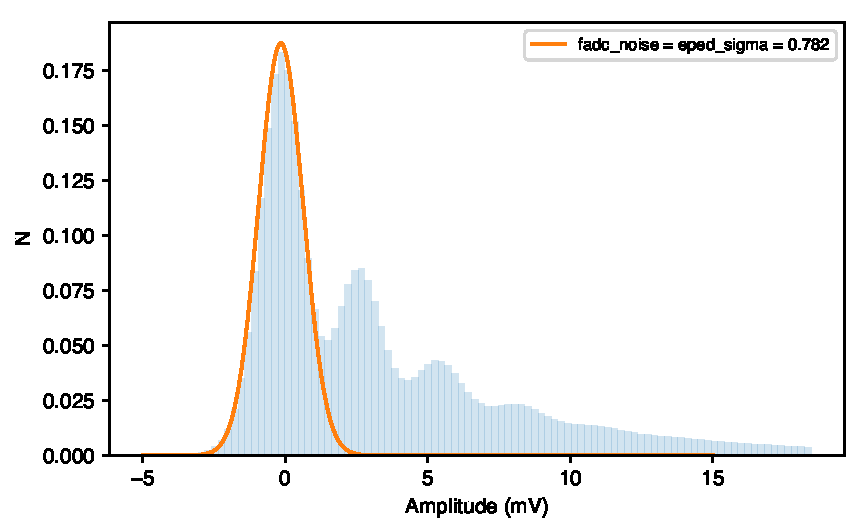
\includegraphics[width=0.55\textwidth]{../38_fadcNoise/checs_fadc_noise_v2.pdf} 
\caption{FADC Noise, measured as the width of the pedestal peak}
\label{fig:fadcnoise}
\end{figure}

\begin{itemize}
\item Gaussian r.m.s. spread of white noise per time bin in digitisation (for high-gain channel, if different gains are used).
\item Value adopted: 0.69
\item Value adopted V2: 1.4 
\item Description of source: See Figure \ref{fig:fadcnoise}. measured as the width of the pedestal peak which provides a value of 0.782. However in simulations to match the SPE spectrum from simulations to that measured in the lab, this has been increased to 1.4.
\item Status: \color{red}Awaiting confermation\color{black}
\item Agreed by: 
\end{itemize}

\section{FADC Max Signal }
\begin{itemize}
\item The maximum value of the digitized signal per sample. For a typical 12-bit ADC this would be 4095.
\item Value adopted: 
\item Description of source: Needs increasing untill we decide how to deal with saturation.
\item Status: 
\item Agreed by: 
\end{itemize}

\section{FADC Pedestal Variation}

\begin{figure}
\centering
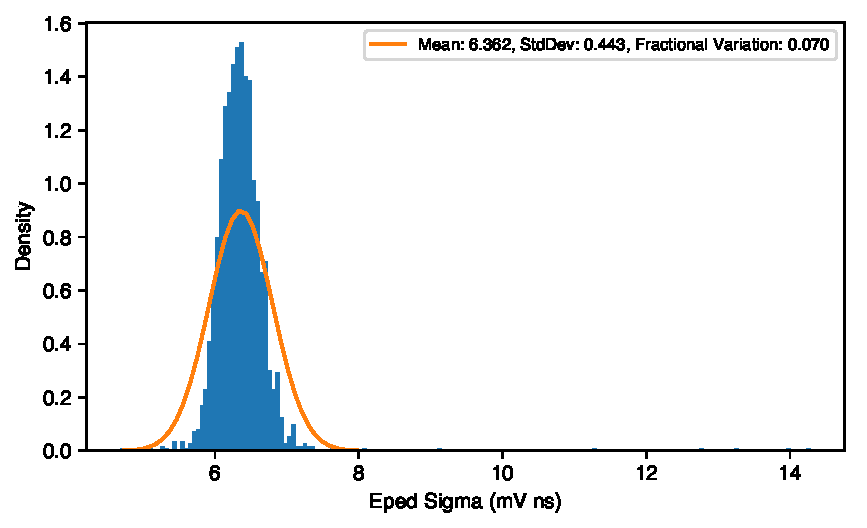
\includegraphics[width=0.55\textwidth]{../40_fadcPedVar/checs_fadc_pedestal_variation_v2.pdf} 
\caption{Variation of pedestal values between pixels}
\label{fig:fadcpedvar}
\end{figure}

\begin{itemize}
\item Channel-to-channel (or pixel-to-pixel) variation of the pedestal per FADC time slice.
\item Value adopted: 10\%
\item Value adopted V2: 7\%
\item Description of source: See Figure \ref{fig:fadcpedvar}. Variation of pedestal values between pixels \color{red} X Needs data description \color{black}
\item Status: \color{red}Awaiting measurement\color{black}
\item Agreed by: 
\end{itemize}

\section{Camera Filter}
\begin{itemize}
\item Wavelength dependence of the camera transmission, independent of the pixel type and the angle of incidence. If a file name is provided, the table (wavelength and efficiency columns) will be loaded and interpolated. The corresponding efficiency factors will be applied on top of the global CAMERA\_TRANSmission factor, and on top of any pixel-type dependent efficiency (both angular and by wavelength), according to the PixType configuration lines in the file specified by CAMERA\_CONFIG\_FILE. The file is, by default, assumed to be a 1-D table (wavelength-dependent only, in nanometers) but, with a\#@RPOL@ header line can be marked and used as a 2-D table (wavelength and angle dependent), with the incidence angles specified in the file in units of degrees but internally converted to radians.
\item Value adopted: 41\_cameraFilter/xtuvt\_ext.dat (prototype, wavelength only)
\item Description of source: Final design currently under investigation, for the prototype a hard coated PMMA window will be used. Data provided is from XT UVT curve in the Polycasa data sheet although has been confirmed by measurements in Liverpool in the available wavelength range (see Figure \ref{fig:window-proto}). It is worth noting, that for any of the validation measurement, the window will not be used. 
\item Status: Under development
\item Agreed by:
\end{itemize}

\begin{figure}
\centering
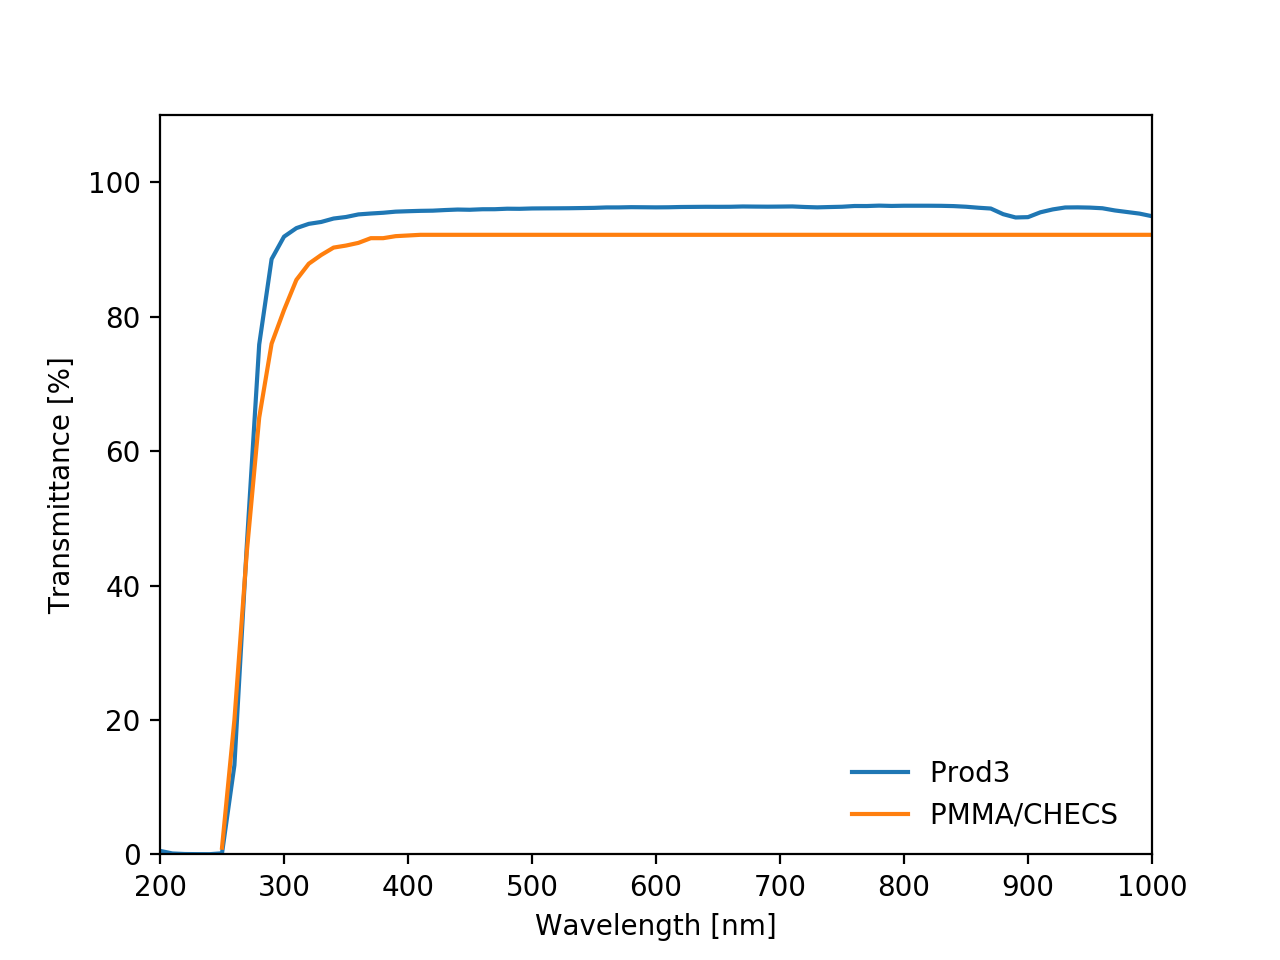
\includegraphics[width=0.55\textwidth]{../41_cameraFilter/PrototypeWavelength.png} 
\caption{prototype window used for CHEC-S.}
\label{fig:window-proto}
\end{figure}

%%%%%%%%%%%%%%%%%%%%%%%%%%%%%%
%%%%% Appendices
%%%%%%%%%%%%%%%%%%%%%%%%%%%%%%
\begin{appendices}

\end{appendices}

%%%%%% DONT CHANGE ! %%%%%%%%%%%%%%%
%\cleardoublepage
\normalsize\small\footnotesize\scriptsize
\addcontentsline{toc}{chapter}{References}
\bibliographystyle{bibgen}
%%%%%%%%%%%%%%%%%%%%%%%%%%%%%%

%%%%%%%%%%%%%%%%%%%%%%%%%%%%%%%%%%%%%%%%%%%%%%
%%%%% Print the References   -   USES BibTeX: UPDATE TO SHOW YOUR .BIB FILES
%%%%%%%%%%%%%%%%%%%%%%%%%%%%%%%%%%%%%%%%%%%%%%%

%\bibliography{C:/Users/Goullon/Documents/BibDocs/AllDocs}		

%%%%% DONT CHANGE ! %%%%%%%%%%%%%
\markboth{}{References}
\normalsize
\glsaddall
\printglossaries
\markboth{}{Glossary}
\end{document}
%%%%%%%%%%%%%%%%%%%%%%%%%%%%
